\section{Auswertung}
\subsection{Wheatstonesche Brücke}
Wir messen folgende Werte für den unbekannten Widerstand $R_x$ mit dem Namen "Wert 10":
\begin{table}
  \centering
  \label{tab:r_10}
  \begin{tabular}{c|cccc}
    \toprule
    & {$R_2 \:/\: \si{\ohm}$} & {$R_3\:/\: \si{\ohm}$} & {$R_4\:/\: \si{\ohm}$} & {$R_x\:/\: \si{\ohm}$} \\
    \midrule
    {Messung 1} & 1000 & 194 & 806 & 240.69 \\
    {Messung 2} & 664 & 265 & 735 & 239.40 \\
    {Messung 3} & 332 & 419 & 581 & 239.43 \\
    \bottomrule
  \end{tabular}
  \caption{Messwerte für den unbekannten Widerstand $R_x$ (Wert 10).}
\end{table}
\\
Nach \eqref{eqn:mittel} und \eqref{eqn:fehler} erhalten wir für $R_x$
\begin{equation*}
  R_x = \SI{239.84(74)}{\ohm}.
\end{equation*}
\\
Für den zweiten unbekannten Widerstand $R_x$ (Wert 12) ergeben sich folgende Widerstände:
\begin{table}
  \centering
  \label{tab:r_12}
  \begin{tabular}{c|cccc}
    \toprule
    & {$R_2 \:/\: \si{\ohm}$} & {$R_3\:/\: \si{\ohm}$} & {$R_4\:/\: \si{\ohm}$} & {$R_x\:/\: \si{\ohm}$} \\
    \midrule
  {Messung 1} & 332 & 540 & 460 & 389.74\\
  {Messung 2} & 1000 & 281 & 719 & 390.82\\
  {Messung 3} &  664 & 370 & 630 & 389.97\\
    \bottomrule
  \end{tabular}
  \caption{Messwerte für den unbekannten Widerstand $R_x$ (Wert 12).}
\end{table}
\\
Wie zuvor für den ersten unbekannten Widerstand berechnet, ergibt sich im Mittel für $R_x$ (Wert 12)
\begin{equation*}
  R_x = \SI{390.17(57)}{\ohm}
\end{equation*}

\subsection{Kapazitätsmessbrücke}
Mit dem Versuchsaufbau der Kapazitätsmessbrücke kann die Kapazität $C_x$ \eqref{eqn:kapc}
eines unbekannten Kondensators mit Verlust $R_x$ \eqref{eqn:abgleich_2} ermittelt werden.
Wir messen folgende Werte:
\begin{table}
  \centering
  \label{tab:b_19}
  \begin{tabular}{c|cccccc}
    \toprule
    & {$C_2 \:/\: \si{\nano \farad}$} & {$R_2\:/\: \si{\ohm}$} & {$R_3\:/\: \si{\ohm}$} & {$R_4\:/\: \si{\ohm}$} & {$R_x\:/\: \si{\ohm}$} & {$C_x \:/\: \si{\nano\farad}$} \\
    \midrule
    {Messung 1} & 750 & 500 & 620 & 380 & 815.79 & 459.68\\
    {Messung 2} & 597 & 500 & 573 & 427 & 670.96 & 444.88\\
    {Messung 3} & 450 & 500 & 508 & 492 & 516.26 & 435.83\\
    \bottomrule
  \end{tabular}
  \caption{Messergbenisse für die unbekannte Kapazität $C_x$ des Kondensators(Wert 19) mit unbekanntem Verlust $R_x$.}
\end{table}
\\
Mit \eqref{eqn:mittel} und \eqref{eqn:fehler} folgt für die Kapazität $C_x$ (Wert 19)
\begin{equation*}
 C_x = \SI{446.80(1204)}{\nano \farad}
\end{equation*}
und für den Widerstand $R_x$
\begin{equation*}
  R_x = \SI{667.67(14979)}{\ohm}.
\end{equation*}
\subsection{Induktivitätsmessbrücke}
Mit den gemessenen Größen $L_2, R_2, R_3, R_4$ und den Formeln \eqref{eqn:indl} und \eqref{eqn:abgleich_2} ergibt sich folgendes für Wert 16:
\begin{table}
  \centering
  \label{tab:c_16}
  \begin{tabular}{c|cccccc}
    \toprule
    & {$L_2 \:/\: \si{\milli\henry}$} & {$R_2\:/\: \si{\ohm}$} & {$R_3\:/\: \si{\ohm}$} & {$R_4\:/\: \si{\ohm}$} & {$R_x\:/\: \si{\ohm}$} & {$L_x \:/\: \si{\milli \henry}$} \\
    \midrule
    {Messung 1} & 20.1 & 332 & 616 & 384 & 532.58 & 12.53\\
    {Messung 2} & 20.1 & 1000 & 270 & 730 & 369.86 & 54.34\\
    {Messung 3} & 20.1 & 500 & 454 & 546 & 415.75 & 24.17\\
    \bottomrule
  \end{tabular}
  \caption{Messergbenisse für die unbekannte Induktivität $L_x$ der Spule(Wert 16) mit unbekanntem Verlust $R_x$.}
\end{table}
\\
Daraus folgt für die gesuchte Induktivität(Wert 16) und den Widerstand
\begin{equation*}
  L_x = \SI{30.35(2158)}{\milli\henry}
\end{equation*}
\begin{equation*}
  R_x = \SI{439.40(8390)}{\ohm}
\end{equation*}
\subsection{Maxwell-Brücke}
In der Tabelle befinden sich die Messwerte für $C_4$, $R_3$, $R_4$ und die daraus resultierenden Werte nach \eqref{eqn:mw_r}
und \eqref{eqn:mw_l} für $R_x$ und $L_x$. Daraus erhalten wir für den gesuchten Widerstand
\begin{equation*}
  R_x = \SI{96.97(836)}{\ohm}
\end{equation*}
und für die gesuchte Induktivität
\begin{equation*}
  L_x = \SI{46.56(1109)}{\milli \henry} .
\end{equation*}
\begin{table}
  \centering
  \label{tab:d_19}
  \begin{tabular}{c|cccccc}
    \toprule
                & {$R_2\:/\: \si{\ohm}$} & {$C_4 \:/\: \si{\nano \farad}$} & {$R_3\:/\: \si{\ohm}$} & {$R_4\:/\: \si{\ohm}$} & {$R_x\:/\: \si{\ohm}$} & {$L_x \:/\: \si{\milli \henry}$} \\
    \midrule
    {Messung 1} & 500 & 399 & 175 & 825 & 106.06 & 34.91 \\
    {Messung 2} & 500 & 597 & 160 & 840 & 95.23 & 47.76 \\
    {Messung 3} & 500 & 750 & 152 & 848 & 89.62 & 57.00 \\
    \bottomrule
  \end{tabular}
  \caption{Messergbenisse für die unbekannte Induktivität $L_x$ der Spule(Wert 19) mit unbekanntem Verlust $R_x$.}
\end{table}
\subsection{Wien-Robinson-Brücke}
In der folgenden Tabelle befinden sich die gemessenen Spannungen $U_\text{Br}$ zu der variierten Frequenz $v \in \left [20, 1000\right ]$.
Das Minimum der Spannung liegt ungefähr bei der Frequenz $v_0 = \SI{160}{\hertz}$. Um das Minimum herum wurde die Spannung in 10-er
 Schritten gemessen, um das Minimum besser darstellen zu können. Die Werte wurden bei einer Speisespannung von $U_\text{S}=\SI{1}{\volt}$ aufgenommen.
\begin{table}
  \centering
  \label{tab:e}
  \begin{tabular}{cc|cc}
    \toprule
    {$v\:/\: \si{\hertz}$} & {$U_\text{Br} \:/\: \si{\milli\volt}$} & {$v\:/\: \si{\hertz}$} & {$U_\text{Br} \:/\: \si{\milli\volt}$} \\
    \midrule
    20 & 252 & 230 & 68 \\
    50 & 188 & 240 & 72 \\
    60 & 168 & 250 & 84 \\
    70 & 148 & 260 & 88 \\
    80 & 136 & 300 & 108 \\
    90 & 120 & 350 & 130 \\
    100 & 84 & 400 & 148 \\
    110 & 68 & 450 & 162 \\
    120 & 52 & 500 & 172 \\
    130 & 36 & 550 & 180 \\
    140 & 24 & 600 & 190 \\
    150 & 12 & 650 & 196 \\
    160 & 8  & 700 & 200 \\
    170 & 20 & 750 & 212 \\
    180 & 28 & 800 & 212 \\
    190 & 40 & 850 & 216 \\
    200 & 48 & 900 & 220 \\
    210 & 56 & 950 & 228 \\
    220 & 60 & 1000 & 228 \\
    \bottomrule
  \end{tabular}
  \caption{Gemessene Spannung $U_\text{Br}$ bei Frequenz $v$ für die Wien-Robinson-Brücke.}
\end{table}
\\
Für die theoretische Berechnung des Minimums, genügt der Widerstand $R$ und die Kapazität $C$.
Dann folgt nach \eqref{eqn:wien_rc} für die Kreisfrequenz
\begin{equation*}
  \omega_0 = \frac{1}{RC} = \frac{1}{993 \cdot 10^{-9}\, \si{\farad} \cdot 1000\, \si{\ohm}} = \SI{1007}{\hertz} 
\end{equation*}
Das bedeutet für das Frequenzverhältnis $\Omega$
\begin{equation*}
  \Omega = \frac{\omega}{\omega_0} = \frac{\omega}{\SI{1007}{\hertz}}
\end{equation*}
mit $\omega=2\pi v$.\\
In der Grafik \ref{fig:plot} ist zum einen das Spannungsverhältnis $\frac{U_\text{Br}}{U_\text{s}}$
und zum anderen die theoretische Kurve \eqref{eqn:wien_verh} zum Frequenzverhältnis $\Omega = v/v_0$ aufgetragen.
\begin{figure}
  \centering
  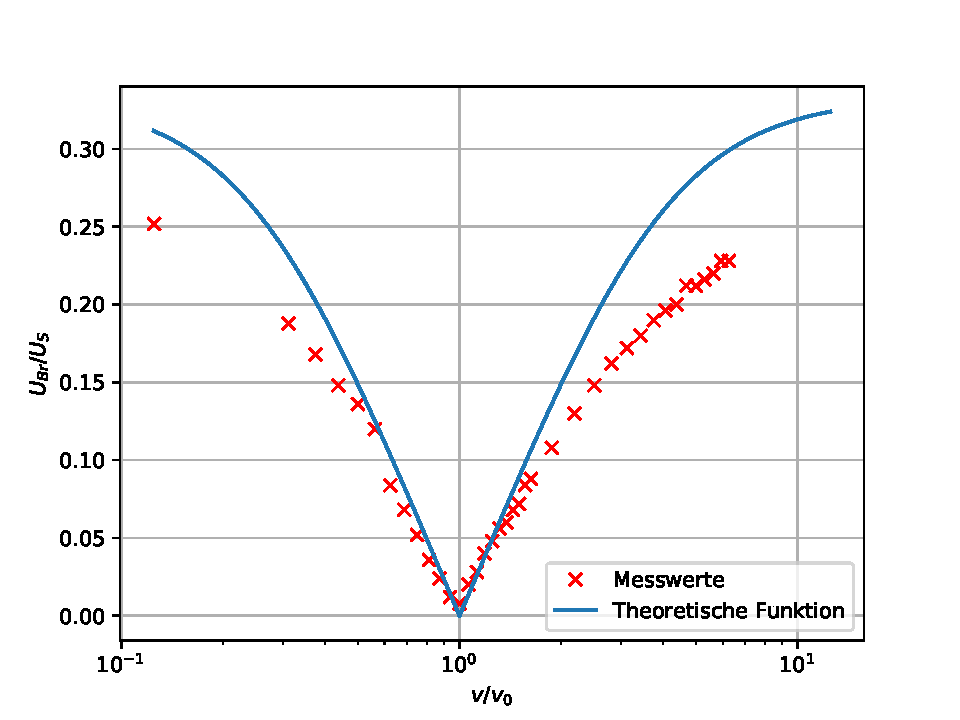
\includegraphics[width=\textwidth]{content/plot_e.pdf}
  \caption{Das gemessene Spannungsverhältnis und die theoretische Kurve zum Vergleich aufgetragen. Der Plot wurde mit dem Python Plugin matplotlib \cite{matplotlib} erstellt.}
  \label{fig:plot}
\end{figure}
\\
Der Klirrfaktor \eqref{eqn:wien_klirr} beschreibt das Verhätnis von den
Oberwellen zur Grundwelle. Hier vereinfachen wir das Problem, indem wir davon ausgehen, dass
die zweite Oberwelle die einzige Oberwelle ist.\\
Es gilt $\Omega = 2$ und für die Effektivspannung der Grundwelle verwenden wir
\begin{equation*}
  U_\text{eff} = \frac{\hat{U}}{\sqrt{2}}
\end{equation*}
und $\hat{U}$ zeitlich gemittelt
\begin{equation*}
  \hat{U} = \frac{1}{2} U
\end{equation*}
Die Effektivspannung im Minimum hat den Wert
\begin{equation*}
  U_\text{eff} = \frac{U}{2 \sqrt{2}} = \SI{2.83}{\milli \volt}.
\end{equation*}
Um die Spannung $U_2$ am Generator zu ermitteln, verwenden wir die Formel für das Spannungsverhältnis \eqref{eqn:verhaeltnis}:
\begin{equation*}
  U_2 = \frac{\SI{2.83}{\milli\volt}}{\sqrt{\frac{1}{9} \frac{(2^2-1)^2}{(1-2^2)^2+9\cdot 2^2}}} = \SI{18.97}{\milli \volt}
\end{equation*}
Der Klirrfaktor mit der Amplitude $U_1=\SI{1}{\volt}$ der Grundwelle, beträgt hier
\begin{equation*}
  k = \frac{U_2}{U_1} = 18.97 \cdot 10^{-3}.
\end{equation*}